% tikz_styles.tex
% TikZ Style Library for Mobile Anyons from Fusion Categories
% ============================================================
% This file provides a comprehensive collection of TikZ styles and macros
% for drawing fusion category diagrams, including:
%   - Fusion trees and morphism diagrams
%   - F-moves (associators) and pentagon equations
%   - R-moves (braiding) and hexagon equations
%   - Evaluation/coevaluation (cups and caps)
%   - Anyon chains and string diagrams

% ============================================================
% Required TikZ Libraries
% ============================================================
\usepackage{tikz}
\usetikzlibrary{
    positioning,           % Relative positioning
    shapes.geometric,      % Geometric shapes
    decorations.markings,  % Arrow decorations on paths
    decorations.pathmorphing, % Wavy/snake lines
    decorations.pathreplacing, % Braces
    arrows,                % Arrow tips
    arrows.meta,           % Modern arrow tips
    knots,                 % Knot crossings for braiding
    calc,                  % Coordinate calculations
    shapes,                % Additional shapes
    backgrounds,           % Background layers
    fit                    % Fitting nodes
}

% ============================================================
% Color Definitions
% ============================================================
% Primary colors for objects/anyons
\definecolor{AnyonRed}{RGB}{221, 6, 0}
\definecolor{AnyonBlue}{RGB}{15, 105, 197}
\definecolor{AnyonGreen}{RGB}{11, 170, 21}
\definecolor{AnyonOrange}{RGB}{238, 143, 0}

% Gray for boxes and backgrounds
\definecolor{LightGray}{RGB}{220,220,220}
\definecolor{MediumGray}{RGB}{180,180,180}

% ============================================================
% Basic Arrow Styles for String Diagrams
% ============================================================
% Arrow at 60% along the path (standard direction)
\tikzset{->-/.style={
    decoration={markings, mark=at position .6 with {\arrow[>=stealth]{>}}},
    postaction={decorate}
}}

% Arrow at 52% (for certain diagram types)
\tikzset{-->--/.style={
    decoration={markings, mark=at position .52 with {\arrow[>=stealth]{>}}},
    postaction={decorate}
}}

% Reverse arrow at 60%
\tikzset{-<-/.style={
    decoration={markings, mark=at position .6 with {\arrow[>=stealth]{<}}},
    postaction={decorate}
}}

% Arrow at 50% (centered)
\tikzset{->>-/.style={
    decoration={markings, mark=at position .5 with {\arrow[>=stealth]{>}}},
    postaction={decorate}
}}

\tikzset{-<<-/.style={
    decoration={markings, mark=at position .5 with {\arrow[>=stealth]{<}}},
    postaction={decorate}
}}

% Arrow at different positions for longer strands
\tikzset{->>>-/.style={
    decoration={markings, mark=at position .5 with {\arrow[>=stealth]{>}}},
    postaction={decorate}
}}

\tikzset{-<<<-/.style={
    decoration={markings, mark=at position .4 with {\arrow[>=stealth]{<}}},
    postaction={decorate}
}}

% ============================================================
% Morphism Box Styles
% ============================================================
% Standard morphism box (gray rounded rectangle)
\tikzset{morphism box/.style={
    rectangle,
    draw,
    rounded corners,
    fill=LightGray,
    text centered,
    minimum height=0.7cm,
    minimum width=0.9cm,
    font=\small
}}

% Small morphism box
\tikzset{morphism box small/.style={
    morphism box,
    minimum height=0.5cm,
    minimum width=0.6cm,
    font=\scriptsize
}}

% Large morphism box (for composite morphisms)
\tikzset{morphism box large/.style={
    morphism box,
    minimum height=1cm,
    minimum width=1.2cm
}}

% ============================================================
% Fusion Vertex Styles
% ============================================================
% Filled vertex (standard trivalent vertex)
\tikzset{fusion vertex/.style={
    circle,
    fill=black,
    inner sep=1.5pt,
    outer sep=0pt
}}

% Empty vertex (for unfilled vertices)
\tikzset{fusion vertex empty/.style={
    circle,
    draw,
    fill=white,
    inner sep=1.5pt,
    outer sep=0pt
}}

% ============================================================
% Label Styles
% ============================================================
% Object labels (on strands)
\tikzset{object label/.style={
    font=\small,
    fill=white,
    inner sep=1pt
}}

% Vertex labels (multiplicity indices at vertices)
\tikzset{vertex label/.style={
    font=\tiny,
    fill=white,
    inner sep=0.5pt
}}

% Coefficient labels (for F-matrices, R-matrices)
\tikzset{coeff label/.style={
    font=\footnotesize,
    midway,
    fill=white,
    inner sep=1pt
}}

% ============================================================
% Commutative Diagram Arrow Style
% ============================================================
\tikzset{cd arrow/.style={
    ->,
    >=stealth,
    thick
}}

% Pentagon/Hexagon diagram arrow
\tikzset{
    pentagon arrow/.style={
        postaction={decorate},
        decoration={markings, mark=at position 1 with {\arrow[scale=1,thick]{>}}}
    }
}

% ============================================================
% MACROS FOR COMMON DIAGRAMS
% ============================================================

% ------------------------------------------------------------
% Trivalent Vertex (splitting): c -> a tensor b
% Usage: \trivalentvertex{a}{b}{c}
% ------------------------------------------------------------
\newcommand{\trivalentvertex}[3]{%
\begin{tikzpicture}[scale=0.7,baseline={(0,0.2)}]
    \draw (0,0) -- +(90:1) node[above] {\small $#3$};
    \draw (0,0) -- +(225:1) node[below] {\small $#1$};
    \draw (0,0) -- +(315:1) node[below] {\small $#2$};
\end{tikzpicture}%
}

% ------------------------------------------------------------
% Left-associative Fusion Tree: ((a,b)_e, c)_d
% Usage: \fuselefttree{a}{b}{e}{c}{d}
% ------------------------------------------------------------
\newcommand{\fuselefttree}[5]{%
\begin{tikzpicture}[scale=0.425,baseline={(0,0.4)}]
    \draw (0,0) node[below] {\small $#1$} -- (1.5,1.5) -- (3,0) node[below] {\small $#4$};
    \draw (0.75,0.75) -- (1.5,0) node[below] {\small $#2$};
    \draw (0.7,1.6) node {\small $#3$};
    \draw (1.5,1.5) -- (1.5,2.25) node[above] {\small $#5$};
\end{tikzpicture}%
}

% ------------------------------------------------------------
% Right-associative Fusion Tree: (a, (b,c)_e)_d
% Usage: \fuserighttree{a}{b}{e}{c}{d}
% ------------------------------------------------------------
\newcommand{\fuserighttree}[5]{%
\begin{tikzpicture}[scale=0.425,baseline={(0,0.4)}]
    \draw (0,0) node[below] {\small $#1$} -- (1.5,1.5) -- (3,0) node[below] {\small $#4$};
    \draw (2.25,0.75) -- (1.5,0) node[below] {\small $#2$};
    \draw (2.3,1.6) node {\small $#3$};
    \draw (1.5,1.5) -- (1.5,2.25) node[above] {\small $#5$};
\end{tikzpicture}%
}

% ------------------------------------------------------------
% F-move (Associator) Equation
% Displays: left tree = sum_f F * right tree
% Usage: \Fmoveequation{a}{b}{c}{d}{e}{f}
% ------------------------------------------------------------
\newcommand{\Fmoveequation}[6]{%
\begin{tikzpicture}[baseline=(current bounding box.center),scale=0.9]
    % Left tree: ((a b)_e c)_d
    \begin{scope}
        \draw (0,0.5) -- (0,1);
        \draw (0,1) -- (-0.5,1.5);
        \draw (-0.5,1.5) -- (-1,2);
        \draw (-0.5,1.5) -- (0,2);
        \draw (0,1) -- (0.5,1.5);
        \draw (0.5,1.5) -- (1,2);
        \node at (0,0.25) {\small $#4$};
        \node at (-1,2.25) {\small $#1$};
        \node at (0,2.25) {\small $#2$};
        \node at (1,2.25) {\small $#3$};
        \node at (-0.5,1.1) {\small $#5$};
    \end{scope}
    % Equals sign
    \node at (1.8,1.25) {$=\displaystyle\sum_{#6} \left(F_{#4}^{#1#2#3}\right)_{#6#5}$};
    % Right tree: (a (b c)_f)_d
    \begin{scope}[xshift=5.5cm]
        \draw (0,0.5) -- (0,1);
        \draw (0,1) -- (-0.5,1.5);
        \draw (-0.5,1.5) -- (-1,2);
        \draw (0.5,1.5) -- (0,2);
        \draw (0,1) -- (0.5,1.5);
        \draw (0.5,1.5) -- (1,2);
        \node at (0,0.25) {\small $#4$};
        \node at (-1,2.25) {\small $#1$};
        \node at (0,2.25) {\small $#2$};
        \node at (1,2.25) {\small $#3$};
        \node at (0.5,1.1) {\small $#6$};
    \end{scope}
\end{tikzpicture}%
}

% ------------------------------------------------------------
% Evaluation (Cup): X* tensor X -> 1
% Usage: \evalcup{X}
% ------------------------------------------------------------
\newcommand{\evalcup}[1]{%
\begin{tikzpicture}[scale=0.85,baseline=(current bounding box.center)]
    \node at (-0.3,0) {$#1^*$};
    \node at (1.7,0) {$#1$};
    \draw (0,0) arc (180:0:0.7);
\end{tikzpicture}%
}

% ------------------------------------------------------------
% Coevaluation (Cap): 1 -> X tensor X*
% Usage: \coevalcap{X}
% ------------------------------------------------------------
\newcommand{\coevalcap}[1]{%
\begin{tikzpicture}[scale=0.85,baseline=(current bounding box.center)]
    \node at (-0.3,0) {$#1$};
    \node at (1.7,0) {$#1^*$};
    \draw (0,0) arc (-180:0:0.7);
\end{tikzpicture}%
}

% ------------------------------------------------------------
% Left Zigzag Identity (Snake equation)
% Usage: \leftzigzag{X}
% ------------------------------------------------------------
\newcommand{\leftzigzag}[1]{%
\begin{tikzpicture}[baseline=(current bounding box.center)]
    \draw (0,0) -- (0,1);
    \draw (0,1) arc (0:180:0.4);
    \draw (-0.8,1) arc (0:-180:0.4);
    \draw (-1.6,1) -- (-1.6,2);
    \node at (0.25,0) {$#1$};
    \node at (-1.85,2) {$#1$};
    \node at (-1.05,1) {$#1^*$};
\end{tikzpicture}%
}

% ------------------------------------------------------------
% Right Zigzag Identity (Snake equation)
% Usage: \rightzigzag{X}
% ------------------------------------------------------------
\newcommand{\rightzigzag}[1]{%
\begin{tikzpicture}[baseline=(current bounding box.center)]
    \draw (0,0) -- (0,1);
    \draw (0,1) arc (180:0:0.4);
    \draw (0.8,1) arc (-180:0:0.4);
    \draw (1.6,1) -- (1.6,2);
    \node at (-0.25,0) {$#1^*$};
    \node at (1.85,2) {$#1^*$};
    \node at (1.05,1) {$#1$};
\end{tikzpicture}%
}

% ------------------------------------------------------------
% Simple Braiding (Over-crossing): X crosses over Y
% Usage: \braidingover{X}{Y}
% ------------------------------------------------------------
\newcommand{\braidingover}[2]{%
\begin{tikzpicture}[scale=0.85,baseline=(current bounding box.center)]
    \node at (-0.75,0.35) {$#1$};
    \node at (-0.75,2.65) {$#2$};
    \node at (0.75,0.35) {$#2$};
    \node at (0.75,2.65) {$#1$};
    \draw (-0.4,0.2) -- (-0.4,0.5);
    \draw (-0.4,2.5) -- (-0.4,2.8);
    \draw (0.4,0.2) -- (0.4,0.5);
    \draw (0.4,2.5) -- (0.4,2.8);
    \begin{knot}[flip crossing/.list={8},consider self intersections=true,ignore endpoint intersections=false]
        \strand (-0.4,0.5)to[out=90,in=270](0.4,2.5);
        \strand (0.4,0.5)to[out=90,in=270](-0.4,2.5);
    \end{knot}
\end{tikzpicture}%
}

% ------------------------------------------------------------
% Inverse Braiding (Under-crossing): X crosses under Y
% Usage: \braidingunder{X}{Y}
% ------------------------------------------------------------
\newcommand{\braidingunder}[2]{%
\begin{tikzpicture}[scale=0.85,baseline=(current bounding box.center)]
    \node at (-0.75,0.35) {$#2$};
    \node at (-0.75,2.65) {$#1$};
    \node at (0.75,0.35) {$#1$};
    \node at (0.75,2.65) {$#2$};
    \draw (-0.4,0.2) -- (-0.4,0.5);
    \draw (-0.4,2.5) -- (-0.4,2.8);
    \draw (0.4,0.2) -- (0.4,0.5);
    \draw (0.4,2.5) -- (0.4,2.8);
    \begin{knot}[flip crossing/.list={8},consider self intersections=true,ignore endpoint intersections=false]
        \strand (0.4,0.5)to[out=90,in=270](-0.4,2.5);
        \strand (-0.4,0.5)to[out=90,in=270](0.4,2.5);
    \end{knot}
\end{tikzpicture}%
}

% ------------------------------------------------------------
% Twist (Ribbon element): curl on a single strand
% Usage: \twist{X}
% ------------------------------------------------------------
\newcommand{\twist}[1]{%
\begin{tikzpicture}[scale=1.1,baseline=(current bounding box.center)]
    \node at (1,0.7)[left] {$#1$};
    \begin{knot}[flip crossing/.list={4,5},consider self intersections=true,ignore endpoint intersections=false]
        \strand (1,0.5)--(1,1);
        \strand (1,1)to[out=90,in=180](1.25,1.75)to[out=0,in=90](1.45,1.5)to[out=270,in=0](1.25,1.25)to[out=180,in=270](1,2);
        \strand (1,2)--(1,2.5);
    \end{knot}
\end{tikzpicture}%
}

% ------------------------------------------------------------
% Bigon (Bubble): a,b fuse to c then split back
% Usage: \bigon{a}{b}{c}
% ------------------------------------------------------------
\newcommand{\bigon}[3]{%
\begin{tikzpicture}[baseline=(current bounding box.center)]
    \draw (0,0) -- (0,0.5);
    \draw (0,0.5) to[bend left=60] node[left] {$#1$} (0,1.5);
    \draw (0,0.5) to[bend right=60] node[right] {$#2$} (0,1.5);
    \draw (0,1.5) -- (0,2);
    \node at (0,-0.25) {$#3$};
    \node at (0,2.25) {$#3$};
\end{tikzpicture}%
}

% ------------------------------------------------------------
% Quantum Dimension Loop: closed loop labeled X
% Usage: \qdimloop{X}
% ------------------------------------------------------------
\newcommand{\qdimloop}[1]{%
\begin{tikzpicture}[baseline=(current bounding box.center)]
    \draw (0,0) circle (0.5cm);
    \node at (0.75,0) {$#1$};
\end{tikzpicture}%
}

% ------------------------------------------------------------
% Identity Strand: straight vertical line
% Usage: \identitystrand{X}
% ------------------------------------------------------------
\newcommand{\identitystrand}[1]{%
\begin{tikzpicture}[baseline=(current bounding box.center)]
    \draw (0,0) -- (0,2);
    \node at (-0.25,0) {$#1$};
    \node at (-0.25,2) {\phantom{$#1$}};
\end{tikzpicture}%
}

% ------------------------------------------------------------
% Anyon Chain Segment: N anyons with fusion labels
% Usage: Place manually or use as template
% ------------------------------------------------------------
\newcommand{\anyonchain}[1]{%
% Draws a simple anyon chain with sites labeled #1
% Customize as needed for specific applications
\begin{tikzpicture}[scale=1.5,baseline=(current bounding box.center)]
    \node at (0,0) {\textbullet};
    \node at (1,0) {\textbullet};
    \node at (2,0) {\textbullet};
    \node at (3,0) {$\cdots$};
    \draw (0.15,0) -- (0.85,0);
    \draw (1.15,0) -- (1.85,0);
    \draw (2.15,0) -- (2.85,0);
    \node at (0,+0.35) {\small $#1_1$};
    \node at (1,+0.35) {\small $#1_2$};
    \node at (2,+0.35) {\small $#1_3$};
\end{tikzpicture}%
}

% ------------------------------------------------------------
% Splitting Tree: General N-particle splitting
% Usage: Manual construction using standard TikZ
% Template provided as example
% ------------------------------------------------------------
% Example usage for 4-particle splitting tree:
% \begin{tikzpicture}[scale=0.8]
%     \draw (0,0) -- (0,0.5);
%     \draw (0,0.5) -- (-0.5,1);
%     \draw (0,0.5) -- (0.5,1);
%     \draw (-0.5,1) -- (-1,1.5);
%     \draw (-0.5,1) -- (0,1.5);
%     \draw (0.5,1) -- (0.5,1.5);
%     \node at (0,-0.25) {$u$};
%     \node at (-1,1.75) {$a$};
%     \node at (0,1.75) {$b$};
%     \node at (0.5,1.75) {$c$};
%     \node at (-0.55,0.7) {\small $e$};
% \end{tikzpicture}

% ============================================================
% Circled Numbers (for numbered items in diagrams)
% ============================================================
\newcommand{\circlednum}[1]{%
\begin{tikzpicture}[baseline={([yshift=-3pt]current bounding box.center)}]
    \node[circle,scale=0.6,draw] at (0,0) {$#1$};
\end{tikzpicture}%
}

\newcommand{\circlednumcolor}[2]{%
\begin{tikzpicture}[baseline={([yshift=-3pt]current bounding box.center)}]
    \node[circle,scale=0.6,draw=#1] at (0,0) {$#2$};
\end{tikzpicture}%
}

% ============================================================
% Diamond Labels (for F-symbol indices)
% ============================================================
\newcommand{\Fdiamond}[1]{%
\begin{tikzpicture}[baseline={([yshift=-3pt]current bounding box.center)},scale=1]
    \node[diamond,scale=0.35,draw,black] at (0,0) {\huge $#1$};
\end{tikzpicture}%
}

% ============================================================
% Temperley-Lieb Patterns
% ============================================================
% Two parallel arcs (TL identity)
\newcommand{\TLidentity}{%
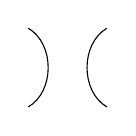
\begin{tikzpicture}[baseline={([yshift=-3pt]current bounding box.center)}]
    \draw (0,0) to [bend right=60] (0,1);
    \draw (1,0) to [bend left=60] (1,1);
\end{tikzpicture}%
}

% Cup-cap pair (TL e_i generator)
\newcommand{\TLcupcap}{%
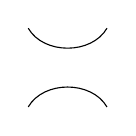
\begin{tikzpicture}[baseline={([yshift=-3pt]current bounding box.center)}]
    \draw (0,0) to [bend left=60] (1,0);
    \draw (0,1) to [bend right=60] (1,1);
\end{tikzpicture}%
}

% H pattern (horizontal connection)
\newcommand{\TLhorizontal}{%
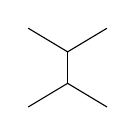
\begin{tikzpicture}[baseline={([yshift=-3pt]current bounding box.center)}]
    \draw (0,0) to (0.5,0.3) to (1,0);
    \draw (0,1) to (0.5,0.7) to (1,1);
    \draw (0.5,0.3) to (0.5,0.7);
\end{tikzpicture}%
}

% ============================================================
% Environment for Full Pentagon Diagram
% ============================================================
% Use the standalone file tex/figures/src/pentagon.tex for the full diagram
% or include inline with the patterns established above.

% ============================================================
% Environment for Full Hexagon Diagram
% ============================================================
% Use the standalone file tex/figures/src/hexagon.tex for the full diagram
% The hexagon.tex in literature/tex provides comprehensive examples.

% ============================================================
% END OF TIKZ STYLE LIBRARY
% ============================================================
